%!TEX root = document.tex

\section{使用示例}

md-highlighter 扩展安装后自动生效,无需操作。以下演示展示了 md-highlighter 扩展在不同分子仿真文件中的语法高亮效果。通过个性化的颜色编码和语义标识,用户可以更高效地编辑和管理各种复杂的分子模拟文件。

\subsection{NAMD/CHARMM 文件格式}

\subsubsection{蛋白质数据库文件(PDB)}

PDB(Protein Data Bank)格式是生物大分子结构数据的国际标准格式。该格式包含了蛋白质、核酸和其他生物大分子的三维原子坐标信息。md-highlighter 为 PDB 文件提供了精细的语法高亮,能够清晰地区分 ATOM、HETATM、REMARK 等不同记录类型,并且对原子坐标、残基信息和链标识符进行颜色编码,大大提高了文件的可读性。

\begin{figure}[!h]
    \centering
    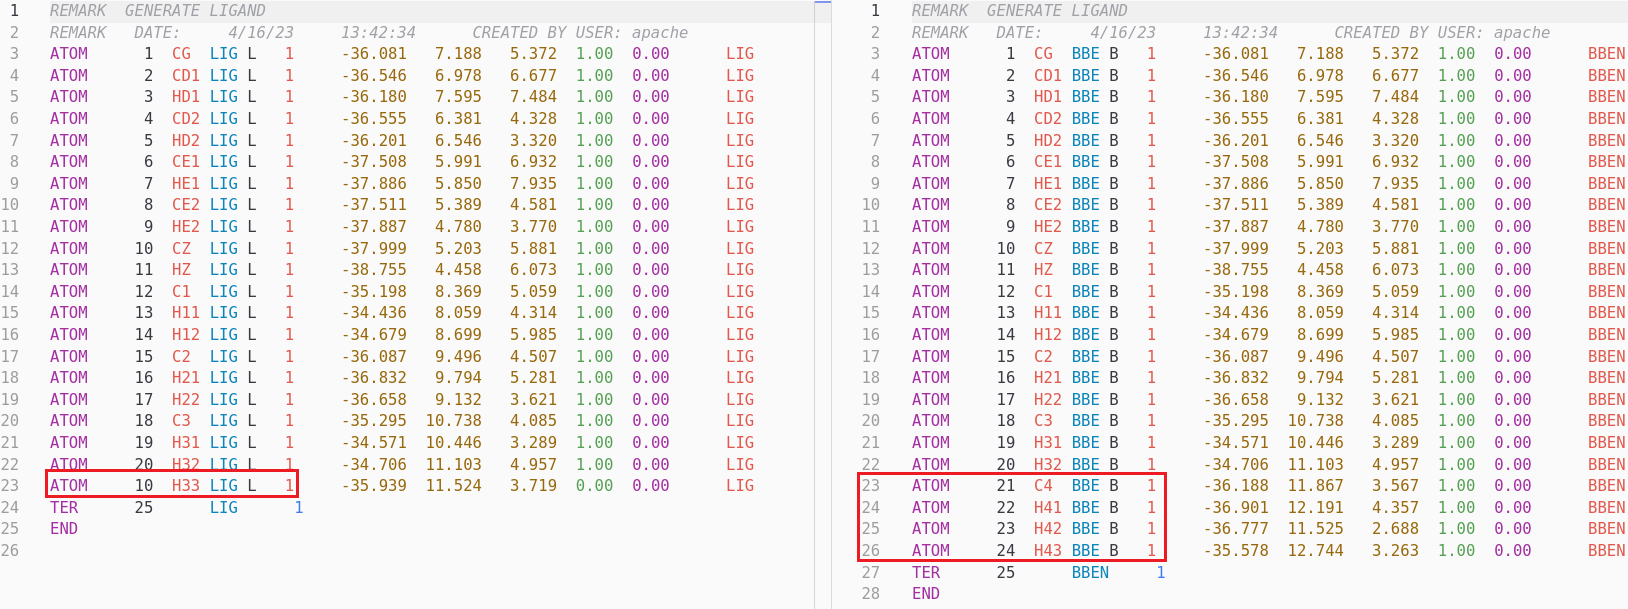
\includegraphics[width=0.85\textwidth]{../images/pdb.png}
    \caption{PDB 文件语法高亮演示(.pdb 格式)}
    \label{fig:pdb-highlighting}
\end{figure}

\textbf{高亮特性:}记录类型、原子坐标、残基信息、链标识符清晰区分

\textbf{应用场景:}结构分析、坐标编辑、格式验证

\subsubsection{残基拓扑文件(RTF)}

RTF(Residue Topology File)文件是 CHARMM 力场中用于定义残基拓扑结构的核心文件。它包含了残基的原子类型、连接关系、电荷分布等关键信息。通过 md-highlighter 的语法高亮,用户可以快速识别 RESI、ATOM、BOND 等关键字,以及各种参数值和注释内容。

\begin{figure}[!h]
    \centering
    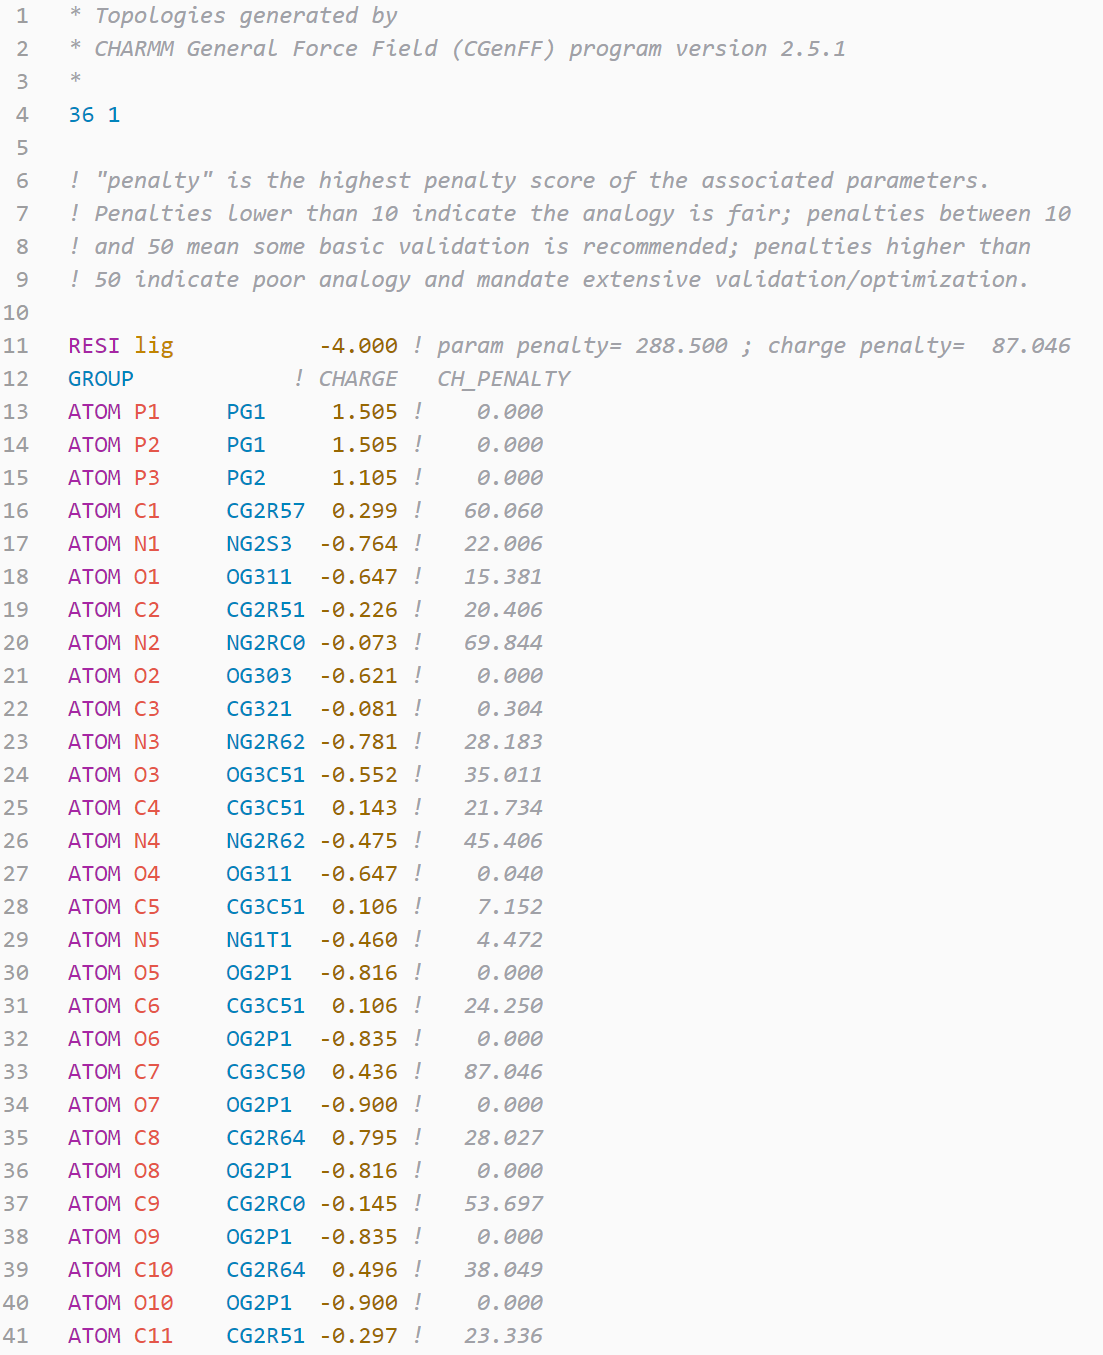
\includegraphics[width=0.85\textwidth]{../images/rtf.png}
    \caption{RTF 文件语法高亮演示(.rtf 格式)}
    \label{fig:rtf-highlighting}
\end{figure}

\textbf{高亮特性:}章节标题、原子定义、连接信息、参数值突出显示

\textbf{应用场景:}力场开发、残基定义、拓扑验证

\subsubsection{蛋白质结构文件(PSF)}

PSF(Protein Structure File)是 NAMD 和 CHARMM 中使用的二进制拓扑文件,存储了分子系统的完整拓扑信息。文件包含原子列表、键连接、角度和二面角定义,是分子动力学模拟的基础文件。md-highlighter 通过对不同章节进行颜色编码,使用户能够快速定位和编辑相关内容。

\begin{figure}[!h]
    \centering
    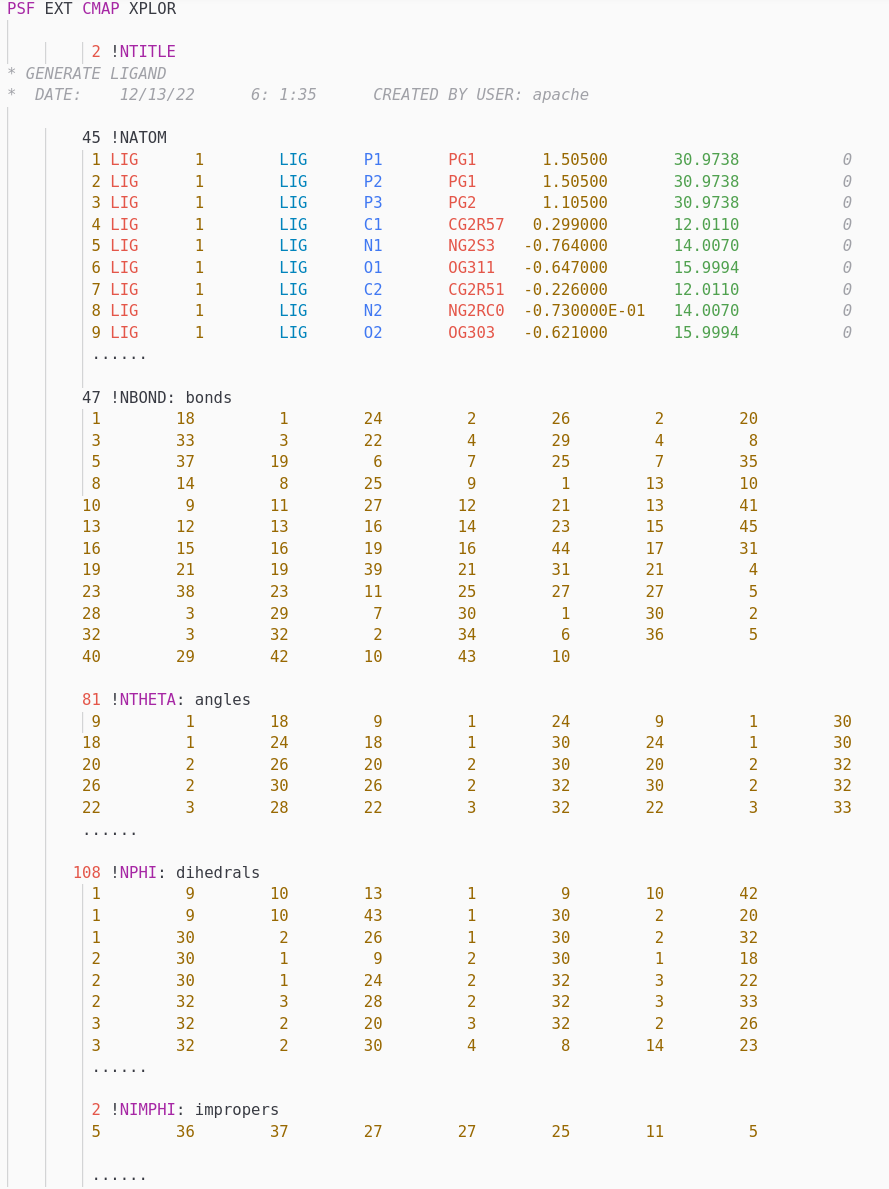
\includegraphics[width=0.85\textwidth]{../images/psf.png}
    \caption{PSF 文件语法高亮演示(.psf 格式)}
    \label{fig:psf-highlighting}
\end{figure}

\textbf{高亮特性:}原子列表、键连接、分子段信息有序组织

\textbf{应用场景:}拓扑验证、连接调试、分子分析

\subsubsection{CHARMM 参数文件(PRM)}

PRM 文件是 NAMD 和 CHARMM 中的参数文件,包含键长、键角、二面角和非键相互作用参数。该文件定义了分子间和分子内相互作用的力学性质,是力场计算的核心组件。md-highlighter 为 PRM 文件提供了清晰的章节区分和参数高亮。

\begin{figure}[!h]
    \centering
    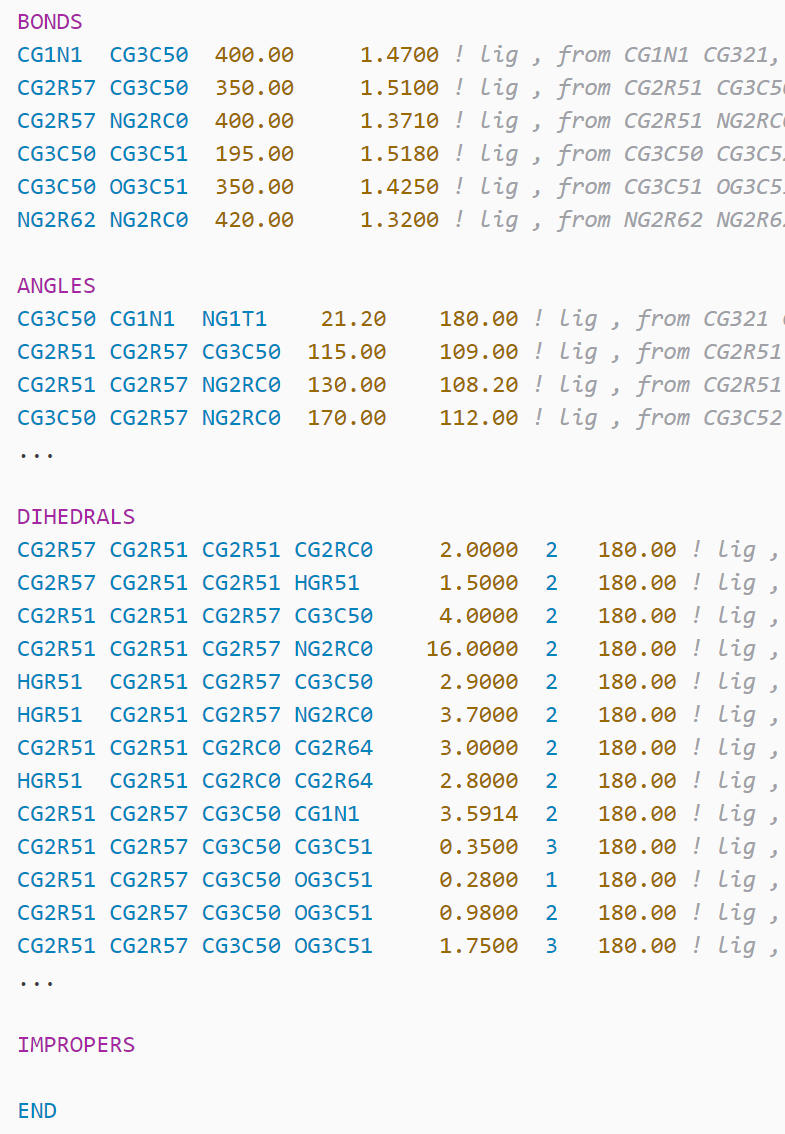
\includegraphics[width=0.85\textwidth]{../images/prm.png}
    \caption{CHARMM PRM 参数文件语法高亮演示(.prm 格式)}
    \label{fig:prm-highlighting}
\end{figure}

\textbf{高亮特性:}参数章节、原子类型、力常数、相互作用定义清晰划分

\textbf{应用场景:}力场开发、参数优化、分子动力学模拟

\subsection{Amber/AmberTools 文件格式}

\subsubsection{Amber 拓扑文件(PRMTOP)}

PRMTOP(Parameter and Topology File)是 Amber 分子动力学软件包中的核心拓扑文件格式。该文件采用特殊的格式化结构,包含了分子系统的全部力场参数和拓扑信息。md-highlighter 能够识别其中的数据块标签、原子信息区域和参数定义,为用户提供清晰的视觉分割。

\begin{figure}[!h]
    \centering
    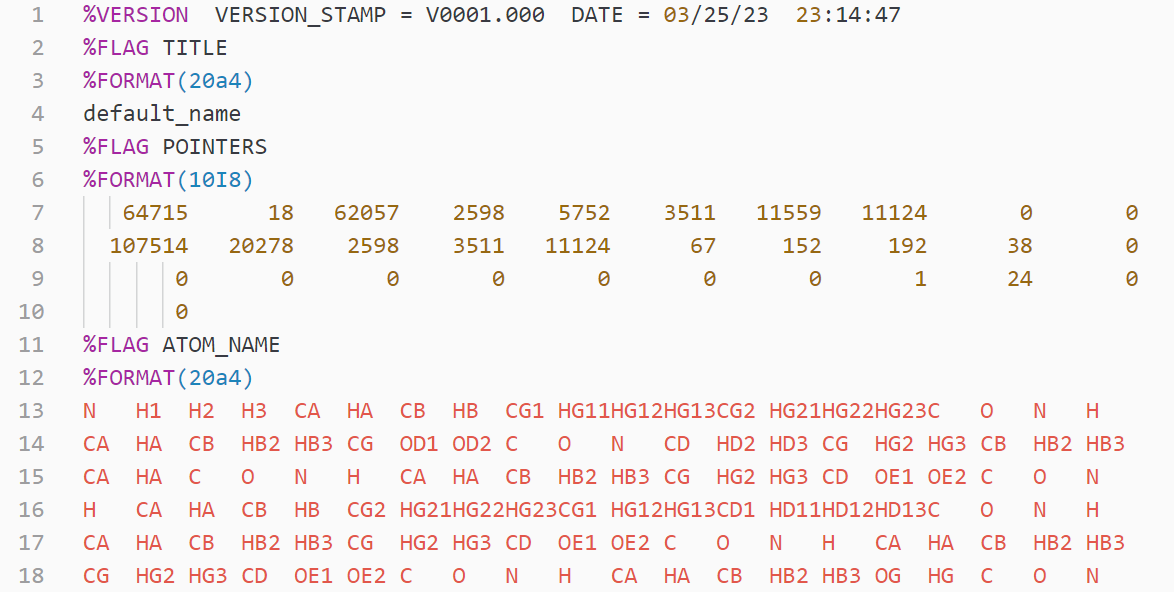
\includegraphics[width=0.85\textwidth]{../images/prmtop.png}
    \caption{Amber PRMTOP 文件语法高亮演示(.prmtop 格式)}
    \label{fig:prmtop-highlighting}
\end{figure}

\textbf{高亮特性:}格式标签、数据块、原子信息、参数区域标识清晰

\textbf{应用场景:}Amber 仿真、拓扑分析、参数验证

\subsubsection{Amber 参数版本7格式 (PARM7)}

PARM7 是 Amber 新版本中使用的拓扑文件格式,与 PRMTOP 功能相似但采用了更加细致的数据组织结构。该格式提供了更好的可读性和更高的数据精度,支持更复杂的分子系统描述。

\begin{figure}[!h]
    \centering
    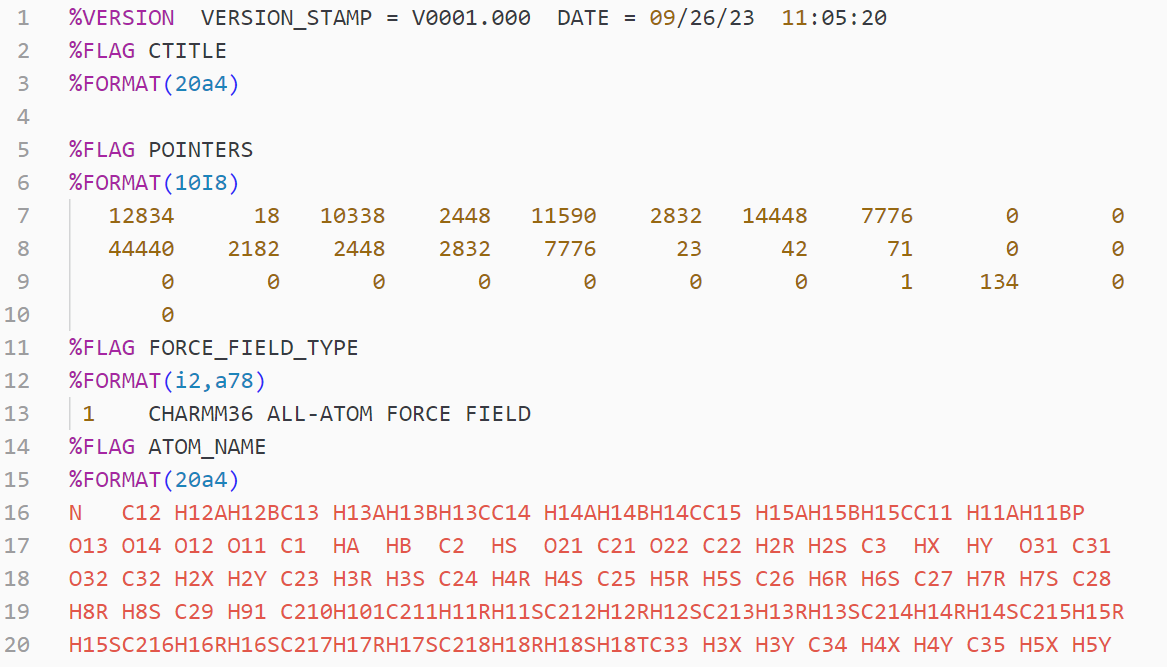
\includegraphics[width=0.85\textwidth]{../images/parm7.png}
    \caption{Amber PARM7 文件语法高亮演示(.parm7 格式)}
    \label{fig:parm7-highlighting}
\end{figure}

\textbf{高亮特性:}数据标签、参数分组、精度指示符、版本信息清晰显示

\textbf{应用场景:}现代 Amber 仿真、高精度计算、跨平台兼容

\subsubsection{Amber 库文件(LIB)}

LIB 文件是 Amber 中用于存储残基库信息的文件格式,包含了原子类型、电荷分布、键连接等详细信息。这种文件在建立复杂分子系统拓扑时起关键作用。md-highlighter 为 LIB 文件提供了精确的语法识别,能够突出显示单元定义、原子列表和库命令。

\begin{figure}[!h]
    \centering
    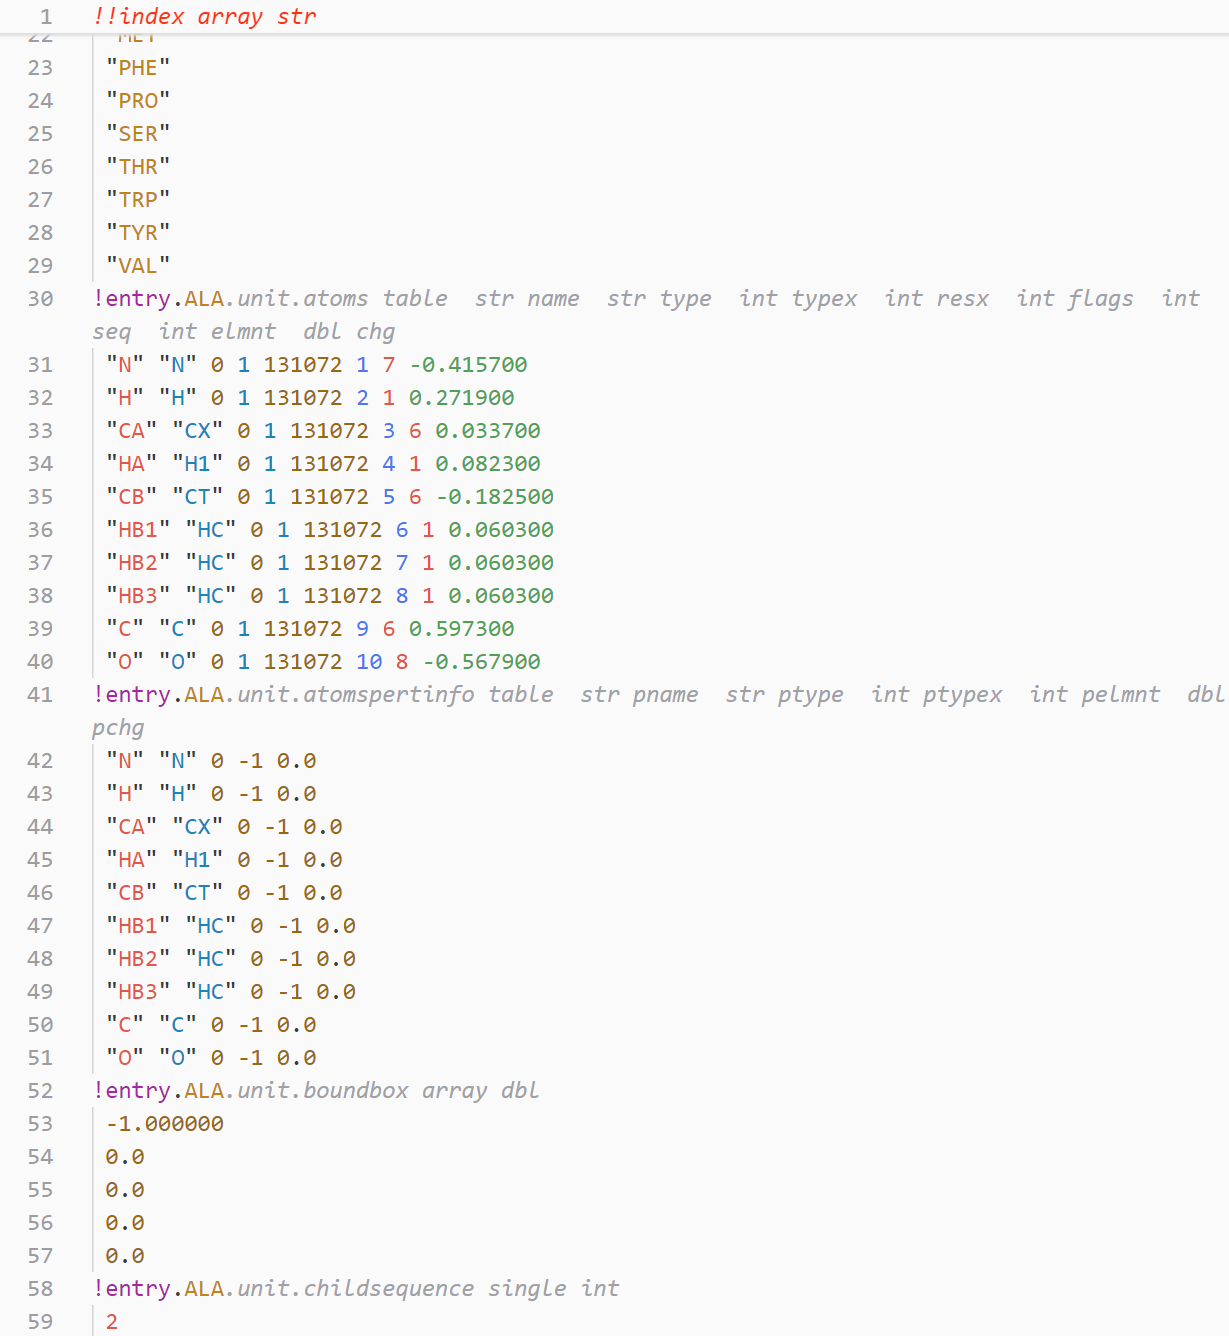
\includegraphics[width=0.65\textwidth]{../images/lib.png}
    \caption{Amber LIB 文件语法高亮演示(.lib 格式)}
    \label{fig:lib-highlighting}
\end{figure}

\textbf{高亮特性:}单元定义、原子列表、连接信息、库命令突出显示

\textbf{应用场景:}库文件开发、残基定义、参数优化

\subsubsection{Amber 预处理输入文件(PREPIN)}

PREPIN 文件是 Amber 中用于定义非标准残基的预处理输入文件。该格式包含残基的几何结构、原子类型、电荷分布和连接信息,用于生成新的残基库条目。md-highlighter 能够识别其中的各种定义区块和参数设置。

\begin{figure}[!h]
    \centering
    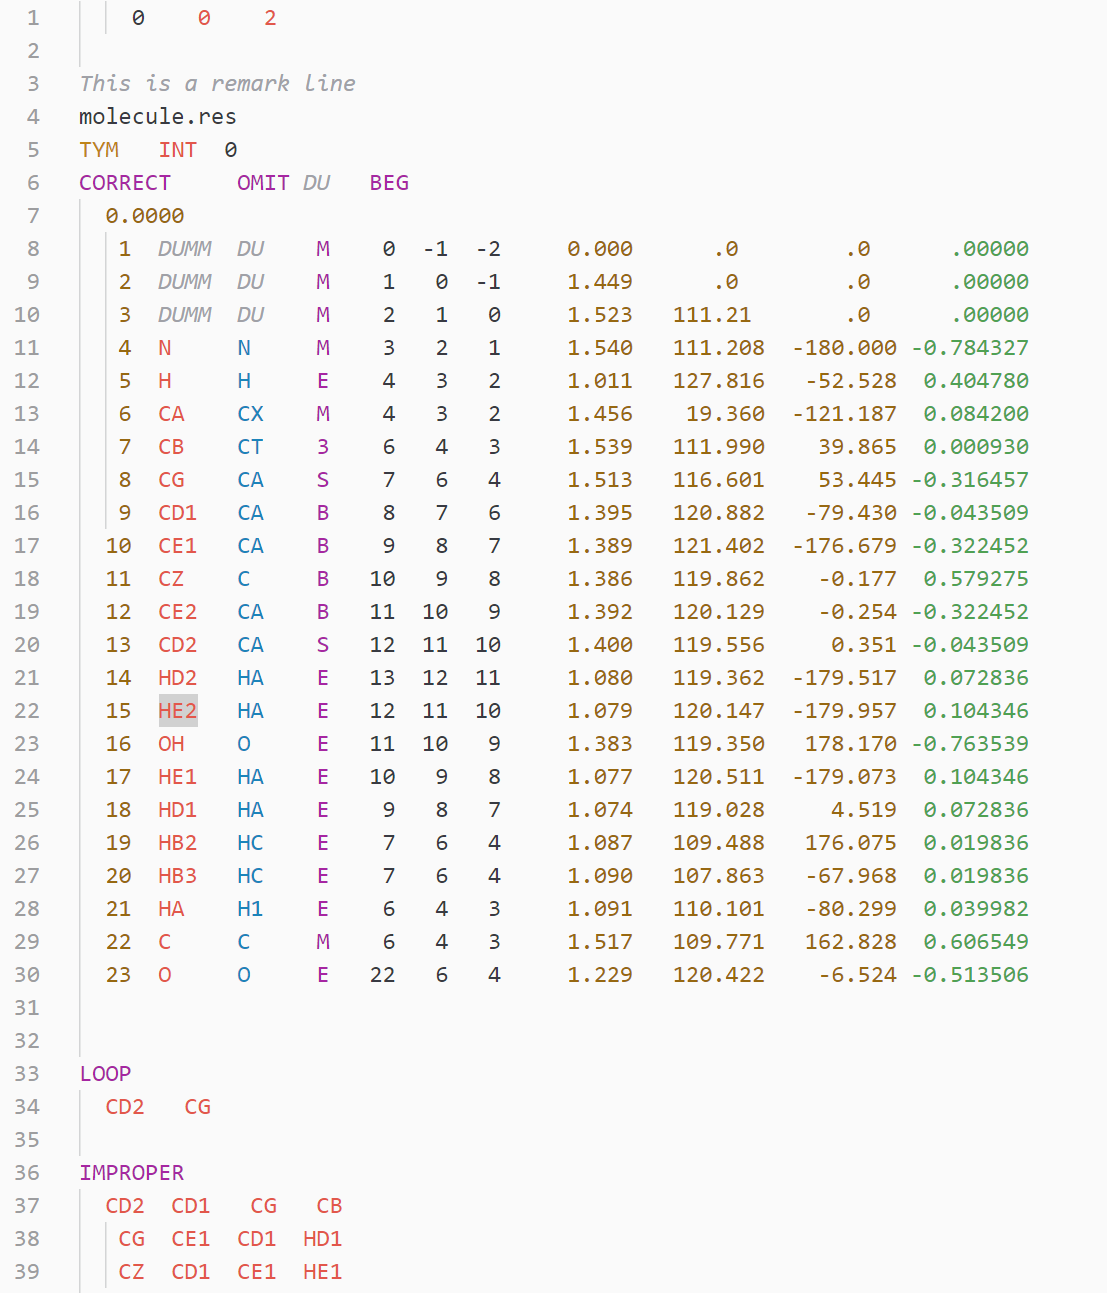
\includegraphics[width=0.65\textwidth]{../images/prepin.png}
    \caption{Amber PREPIN 文件语法高亮演示(.prepin 格式)}
    \label{fig:prepin-highlighting}
\end{figure}

\textbf{高亮特性:}残基定义、原子坐标、电荷分配、连接关系突出显示

\textbf{应用场景:}非标准残基建模、残基库扩展、参数化工作

\subsubsection{Amber 力场修改文件(FRCMOD)}

FRCMOD 文件用于修改或扩展现有的 Amber 力场参数。该文件格式允许用户添加新的原子类型、修改现有参数或定义新的相互作用项。md-highlighter 提供了清晰的参数分类和数值高亮。

\begin{figure}[!h]
    \centering
    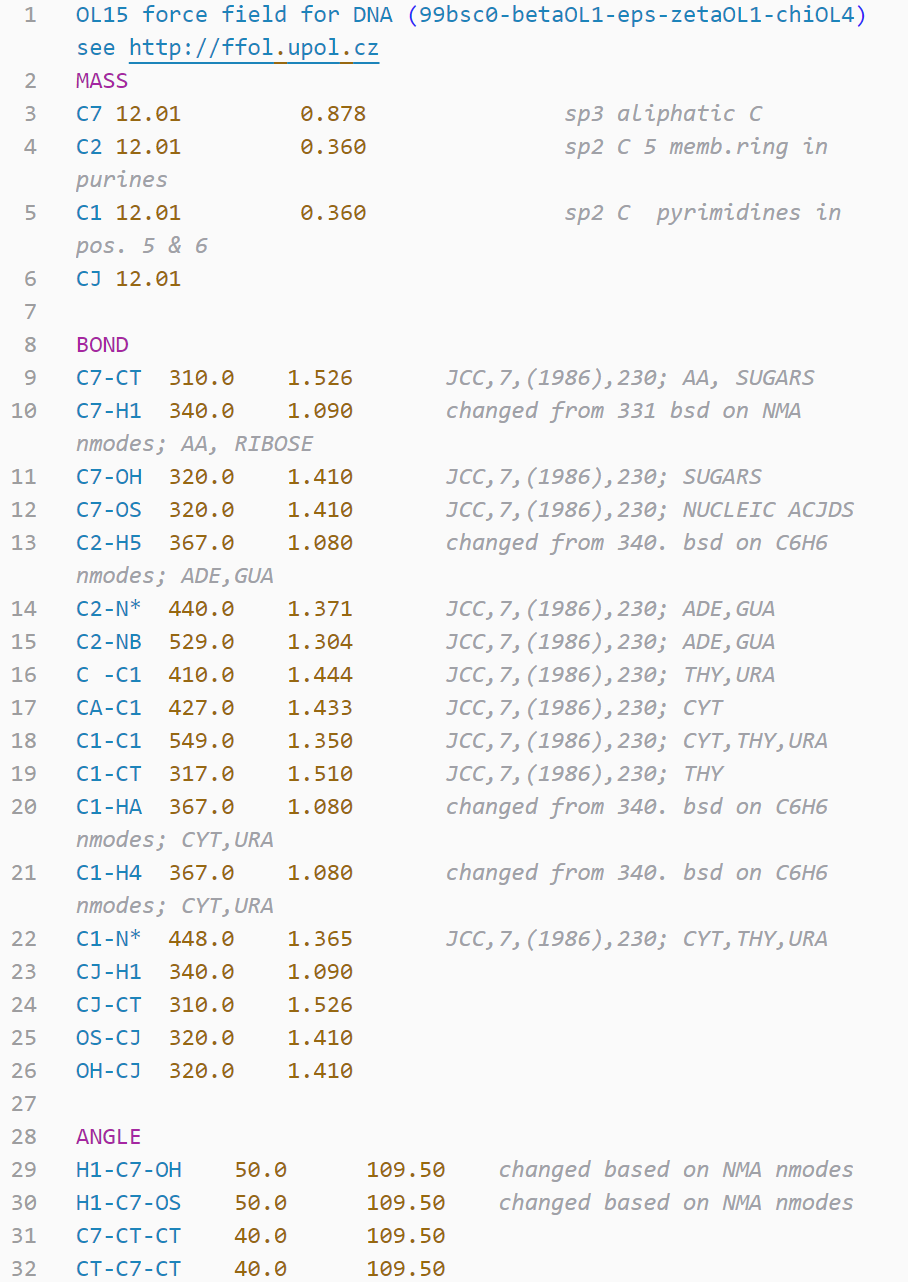
\includegraphics[width=0.65\textwidth]{../images/frcmod.png}
    \caption{Amber FRCMOD 文件语法高亮演示(.frcmod 格式)}
    \label{fig:frcmod-highlighting}
\end{figure}

\textbf{高亮特性:}参数修改、原子类型定义、力场扩展信息清晰组织

\textbf{应用场景:}力场定制、参数微调、新分子类型支持

\subsubsection{AmberTools 输入脚本(TLEAP.IN)}

tleap.in 文件是 AmberTools 中 tleap 程序的输入脚本,用于构建分子系统的拓扑结构。该脚本包含加载力场、添加分子、定义系统等命令序列。md-highlighter 能够识别命令关键字、文件路径和参数设置。

\begin{figure}[!h]
    \centering
    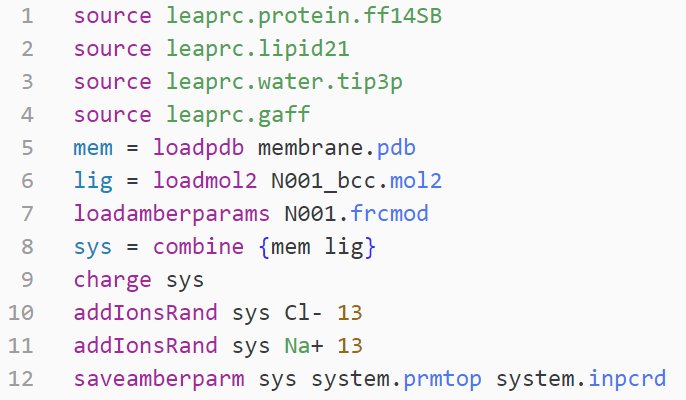
\includegraphics[width=0.8\textwidth]{../images/tleap.in.png}
    \caption{tleap 输入脚本语法高亮演示(.in 格式)}
    \label{fig:tleap-highlighting}
\end{figure}

\textbf{高亮特性:}命令关键字、文件路径、参数值、注释信息清晰区分

\textbf{应用场景:}系统构建、拓扑生成、批处理脚本

\subsubsection{Antechamber 主链文件(MC)}

MC 文件是 Antechamber 工具中用于定义分子主链结构的文件格式。该文件包含主链原子的标识、连接关系和几何信息,用于分子的自动参数化过程。

\begin{figure}[!h]
    \centering
    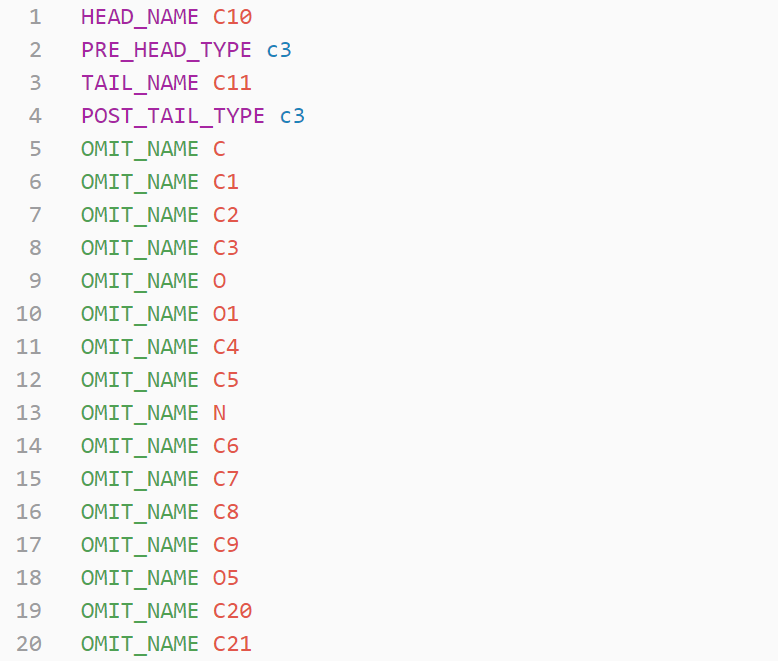
\includegraphics[width=0.7\textwidth]{../images/mc.png}
    \caption{MC 主链文件语法高亮演示(.mc 格式)}
    \label{fig:mc-highlighting}
\end{figure}

\textbf{高亮特性:}主链定义、原子标识、连接信息有序显示

\textbf{应用场景:}小分子参数化、主链识别、结构分析

\subsubsection{Antechamber 文件(AC)}

AC 文件是 Antechamber 工具生成的中间格式文件,主要用于小分子的电荷计算和原子类型分配。该格式包含了分子的原子连接信息、电荷分布和分子描述符。md-highlighter 可以清晰地显示这些不同类型的信息,帮助用户进行小分子参数化工作。

\begin{figure}[!h]
    \centering
    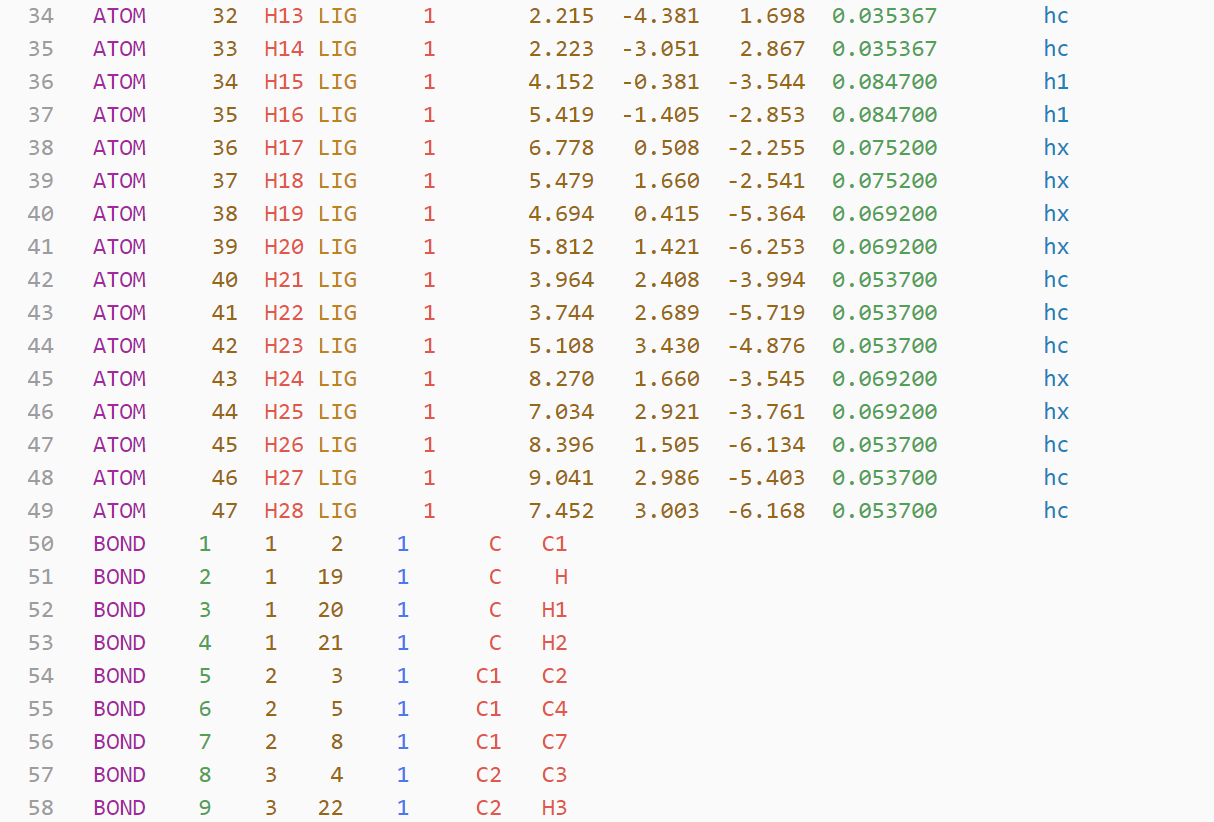
\includegraphics[width=0.85\textwidth]{../images/ac.png}
    \caption{AC 文件语法高亮演示(.ac 格式)}
    \label{fig:ac-highlighting}
\end{figure}

\textbf{高亮特性:}原子连接、电荷信息、分子描述符清晰组织

\subsection{Gromacs 文件格式}

\subsubsection{Gromacs 坐标文件(GRO)}

GRO 文件是 Gromacs 分子动力学软件包中的标准坐标文件格式。与传统的 PDB 格式相比,GRO 格式提供了更高的精度和更紧凑的数据结构。该格式包含原子编号、残基信息、坐标数据和可选的速度信息。md-highlighter 为 GRO 文件提供了精确的语法分析,能够清晰地区分各个数据列。

\begin{figure}[!h]
    \centering
    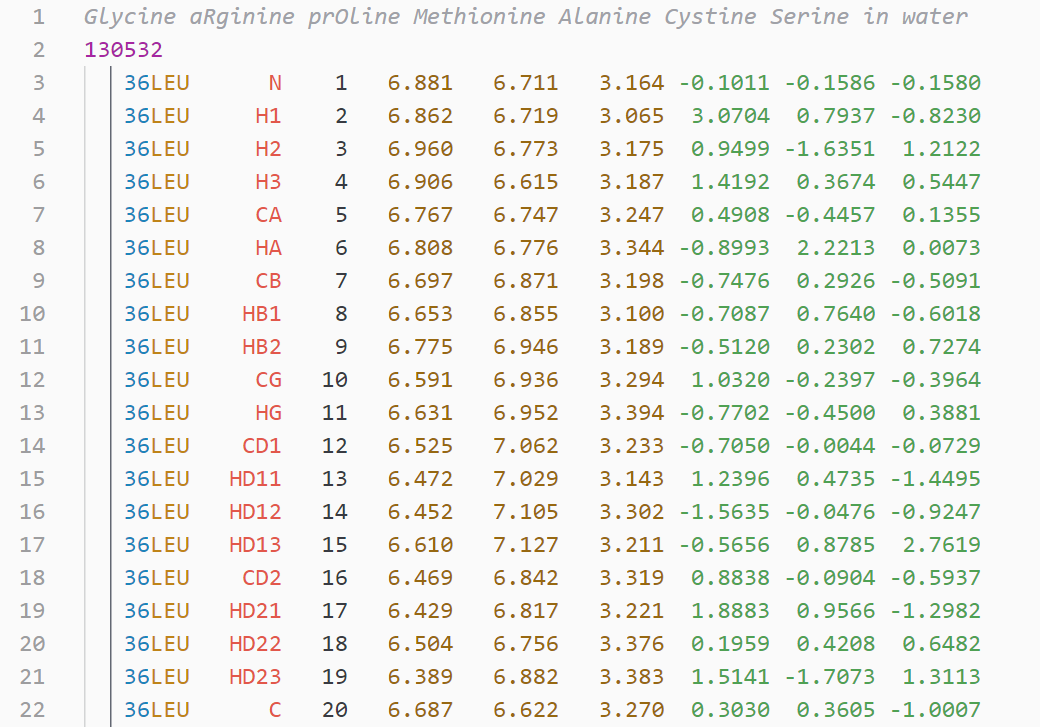
\includegraphics[width=0.8\textwidth]{../images/gro.png}
    \caption{Gromacs GRO 文件语法高亮演示(.gro 格式)}
    \label{fig:gro-highlighting}
\end{figure}

\textbf{高亮特性:}原子编号、残基信息、坐标数据、速度信息清晰划分

\textbf{应用场景:}Gromacs 仿真、坐标分析、轨迹处理

\subsubsection{Gromacs 原子类型文件(ATP)}

ATP 文件定义了 Gromacs 中的原子类型参数,包括原子质量、电荷、原子半径等物理属性。该文件是 Gromacs 力场定义的基础组件,在构建拓扑文件时起关键作用。

\begin{figure}[!h]
    \centering
    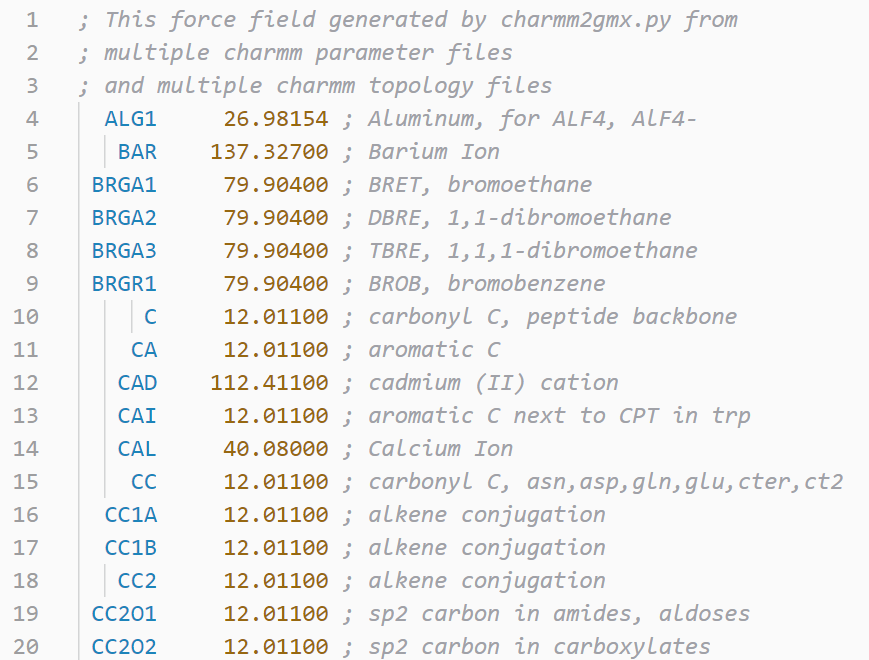
\includegraphics[width=0.8\textwidth]{../images/atp.png}
    \caption{Gromacs ATP 原子类型文件语法高亮演示(.atp 格式)}
    \label{fig:atp-highlighting}
\end{figure}

\textbf{高亮特性:}原子类型名称、质量数据、电荷信息、物理参数清晰分类

\textbf{应用场景:}力场开发、原子类型定义、参数优化

\subsubsection{Gromacs 突变拓扑文件(MTP)}

MTP 文件用于 Gromacs 中的自由能计算,定义了在突变过程中如何修改分子的拓扑结构。该文件包含了初始状态、最终状态和中间状态的定义,支持复杂的化学变化模拟。

\subsubsection{Gromacs 终端数据库文件(TDB)}

TDB 文件定义了 Gromacs 中蛋白质终端的处理方式,包括 N-终端和 C-终端的质子化状态和特殊修饰。该文件在构建蛋白质系统拓扑时提供终端处理的标准化规则。

\begin{figure}[!h]
    \centering
    \begin{subfigure}[c]{0.49\textwidth}
        \centering
        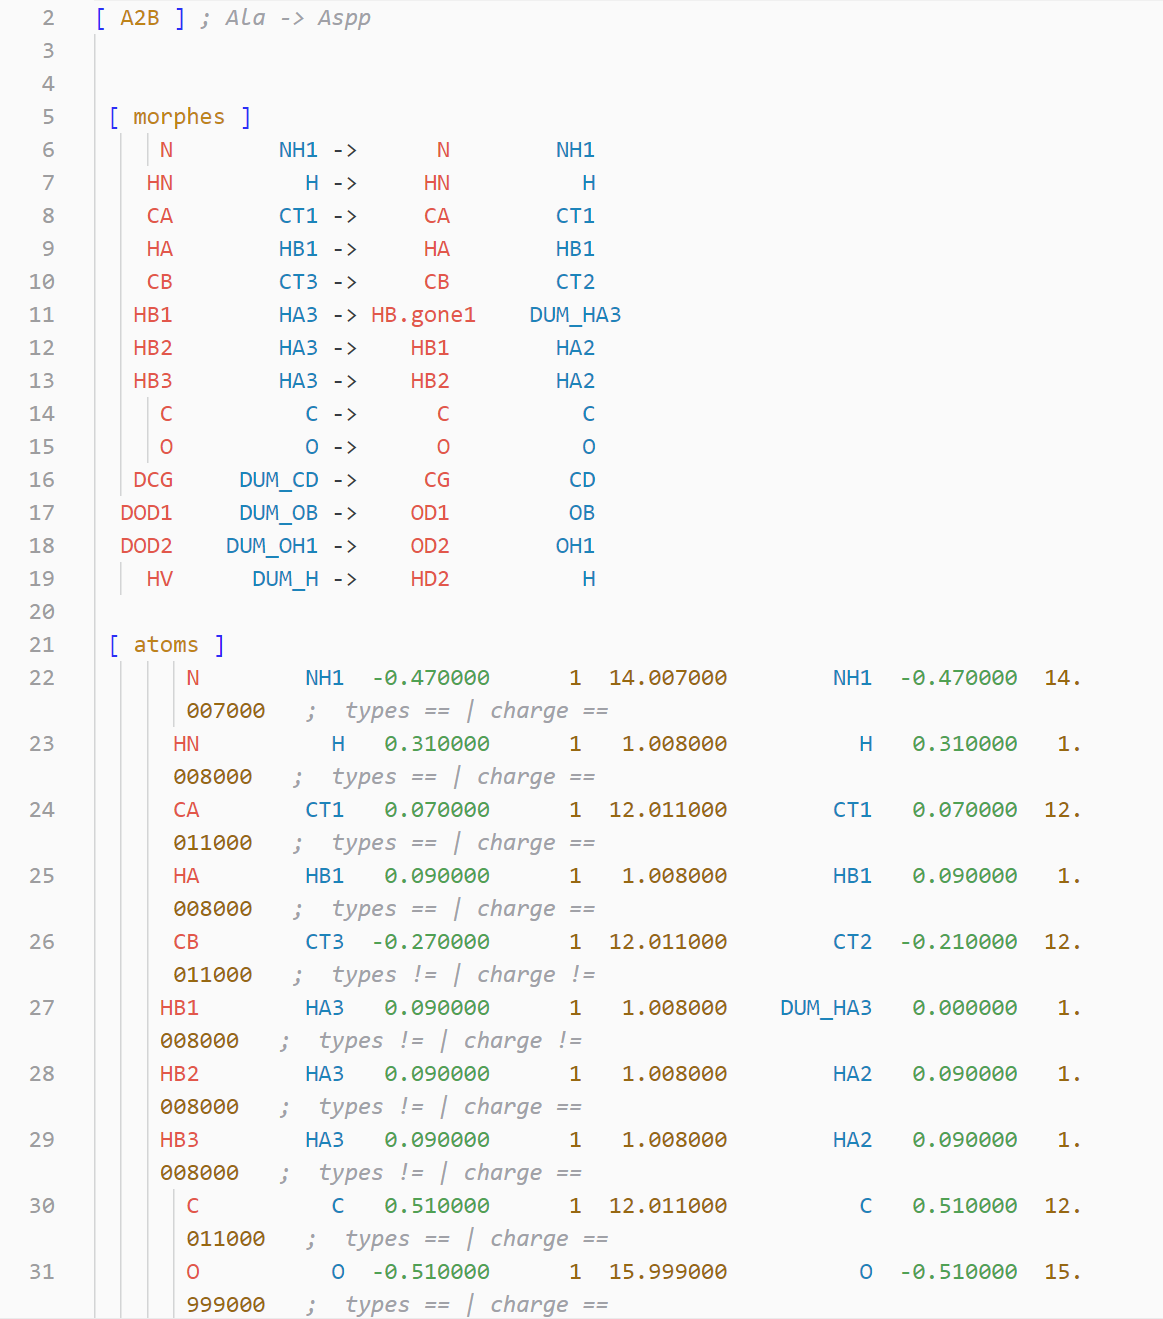
\includegraphics[width=\textwidth]{../images/mtp.png}
        \caption{MTP 格式}
        \label{fig:mtp-highlighting}
    \end{subfigure}
    \hfill
    \begin{subfigure}[c]{0.49\textwidth}
        \centering
        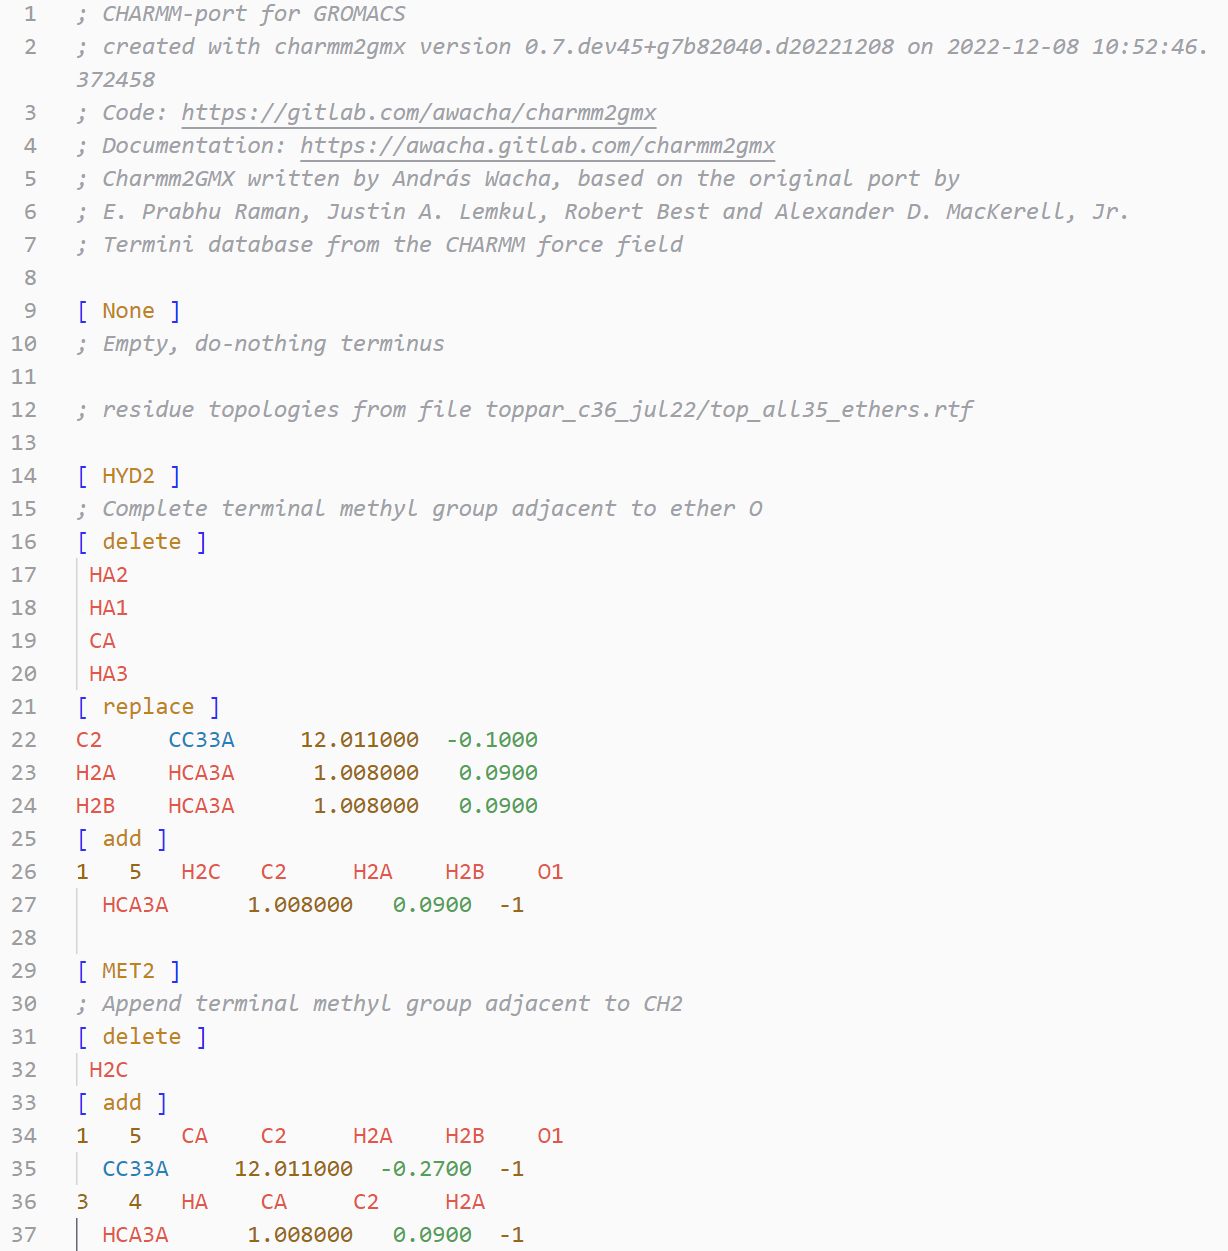
\includegraphics[width=\textwidth]{../images/tdb.png}
        \caption{TDB 格式}
        \label{fig:tdb-highlighting}
    \end{subfigure}
    \caption{Gromacs MTP 突变拓扑文件和 TDB 终端数据库文件语法高亮演示}
    \label{fig:mtp-tdb-highlighting}
\end{figure}

\textbf{MTP高亮特性:}状态定义、拓扑变化、参数转换、突变路径清晰标识

\textbf{MTP应用场景:}自由能计算、突变模拟、化学反应研究

\textbf{TDB高亮特性:}终端类型、修饰定义、质子化状态、原子添加规则清晰分类

\textbf{TDB应用场景:}蛋白质建模、pH 效应模拟、终端修饰研究

\subsection{小分子文件格式}

\subsubsection{MOL2 分子结构文件(MOL2)}

MOL2 是 Tripos 公司开发的小分子结构文件格式,在药物设计和分子建模领域广泛使用。该格式能够存储分子的完整信息,包括原子坐标、电荷分布、原子类型和键连接关系。md-highlighter 为 MOL2 文件提供了细致的语法高亮,能够突出显示不同的数据块和关键信息。

\subsubsection{结构数据文件(SDF)}

SDF(Structure Data File)是化学信息学中广泛使用的分子结构数据格式。该格式能够存储多个分子的结构信息,包括原子坐标、键连接、立体化学信息和分子属性数据。SDF 文件在药物发现和化学数据库管理中应用广泛。

\begin{figure}[!h]
    \centering
    \begin{subfigure}[c]{0.49\textwidth}
        \centering
        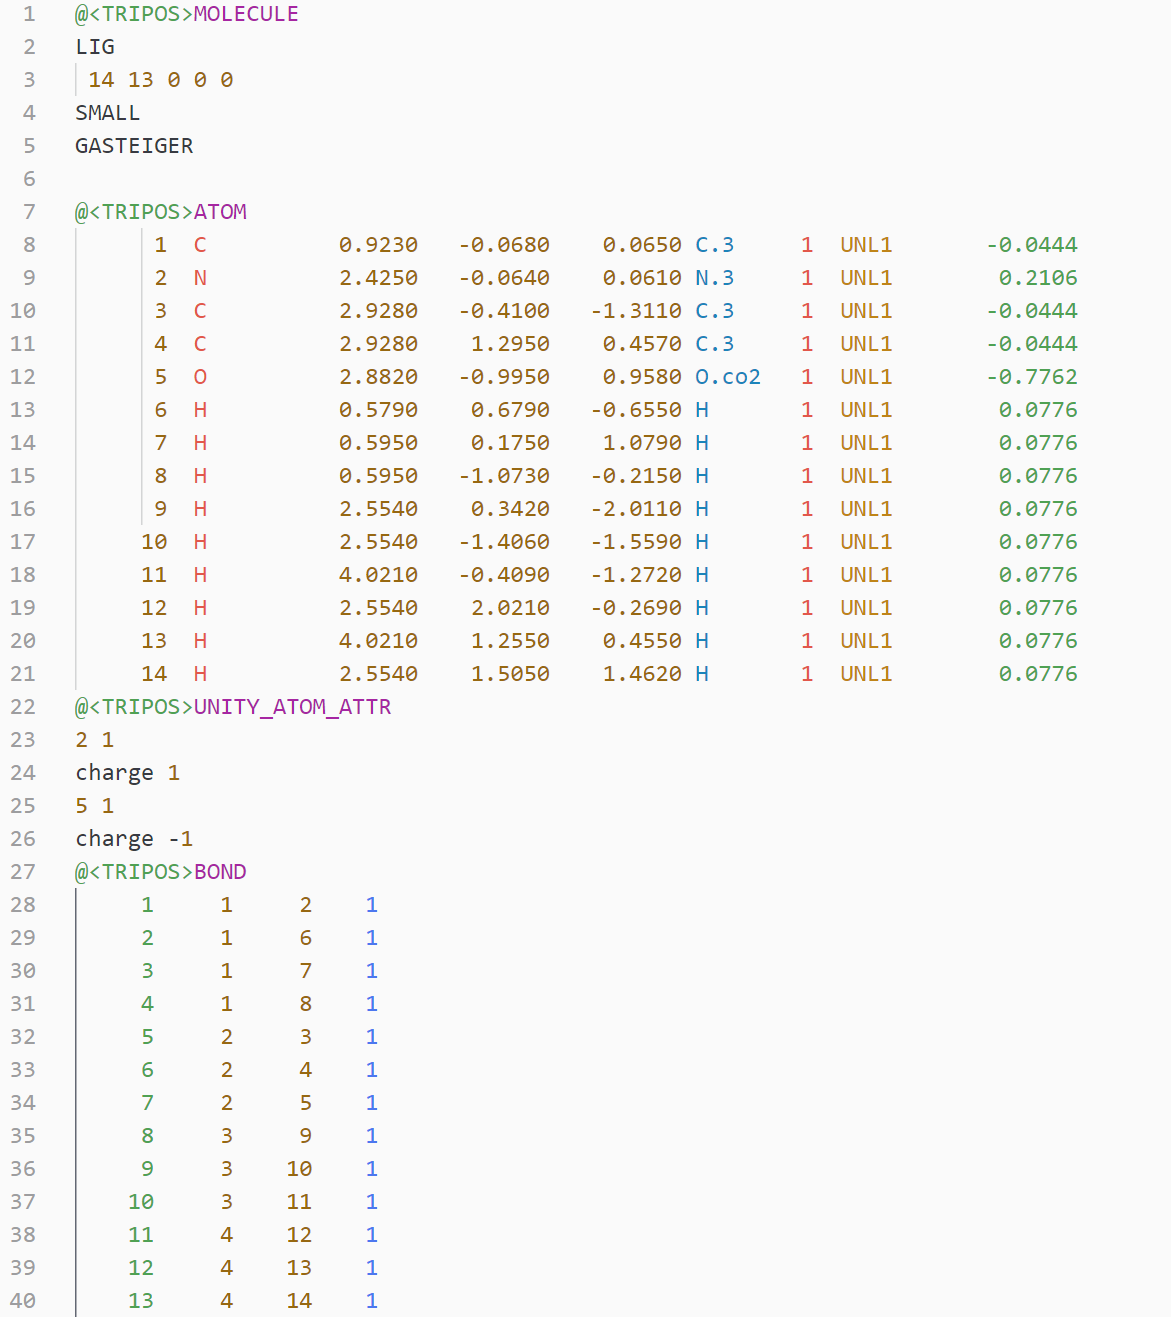
\includegraphics[width=\textwidth]{../images/mol2.png}
        \caption{MOL2 格式}
        \label{fig:mol2-highlighting}
    \end{subfigure}
    \hfill
    \begin{subfigure}[c]{0.49\textwidth}
        \centering
        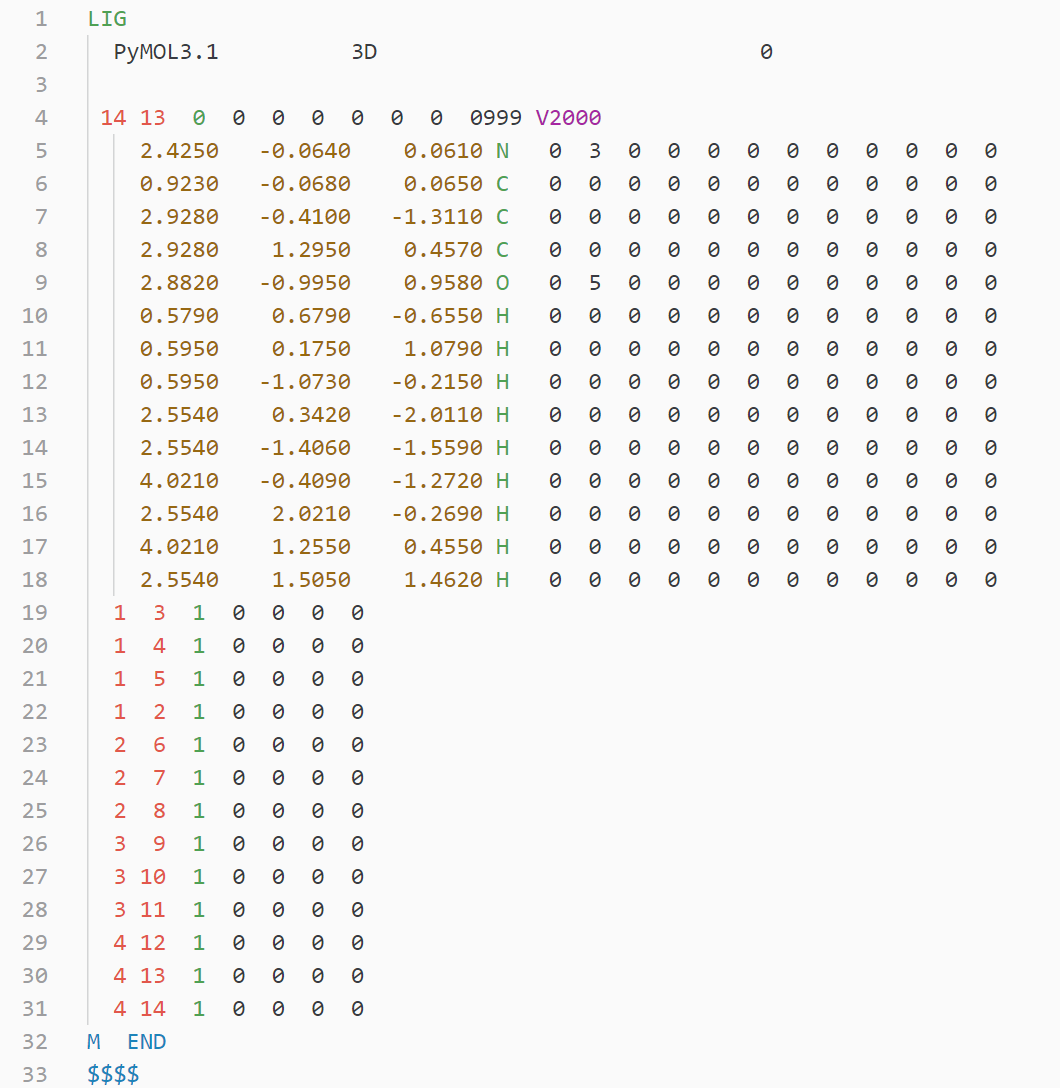
\includegraphics[width=\textwidth]{../images/sdf.png}
        \caption{SDF 格式}
        \label{fig:sdf-highlighting}
    \end{subfigure}
    \caption{MOL2 分子结构文件和 SDF 结构数据文件语法高亮演示}
    \label{fig:mol2-sdf-highlighting}
\end{figure}

\textbf{MOL2高亮特性:}分子信息、原子类型、键连接、电荷数据突出显示

\textbf{MOL2应用场景:}小分子建模、药物设计、化学结构分析

\textbf{SDF高亮特性:}分子数据块、原子坐标、键连接表、属性信息清晰组织

\textbf{SDF应用场景:}化学数据库、药物筛选、分子属性分析

\subsection{增强采样文件格式}

\subsubsection{PLUMED 输入文件}

PLUMED 是一个功能强大的增强采样库,广泛用于分子动力学模拟中的自由能计算和集体变量分析。PLUMED 输入文件使用特殊的语法结构,包含关键字、变量定义、函数参数和注释信息。md-highlighter 能够准确识别这些不同的语法元素,帮助用户更高效地编写和调试 PLUMED 脚本。

\begin{figure}[!h]
    \centering
    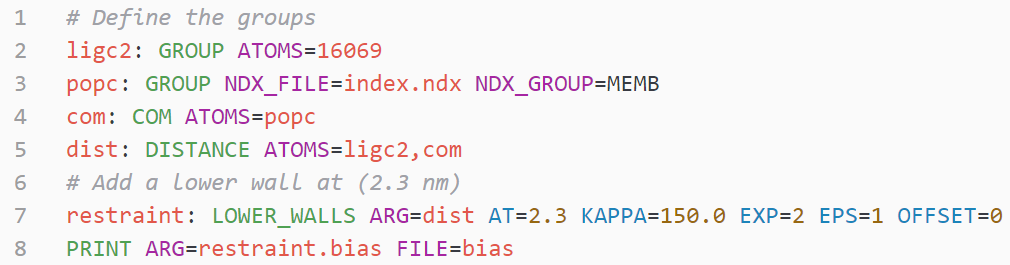
\includegraphics[width=0.85\textwidth]{../images/plumed.png}
    \caption{PLUMED 输入文件语法高亮演示(.plumed.dat 格式)}
    \label{fig:plumed-highlighting}
\end{figure}

\textbf{高亮特性:}关键字、变量定义、函数参数、注释清晰区分

\textbf{应用场景:}增强采样、集体变量定义、自由能计算

\subsection{实际应用指南}

\subsubsection{文件格式验证与调试}
通过语法高亮快速定位文件格式问题:
\begin{itemize}
    \item 识别格式不正确的坐标数据
    \item 发现缺失的原子类型定义
    \item 验证残基编号的连续性
    \item 检查键连接的完整性
\end{itemize}

\subsubsection{跨格式工作流}
md-highlighter 支持完整的分子模拟工作流:
\begin{itemize}
    \item PDB $\to$ PSF $\to$ 参数文件的 NAMD 流程
    \item PDB $\to$ GRO $\to$ TOP 的 Gromacs 流程  
    \item MOL2 $\to$ AC $\to$ PRMTOP 的 Amber 流程
    \item PLUMED 集成的增强采样流程
\end{itemize}

\section{未来发展}

\subsection{计划增强}

md-highlighter 扩展持续发展,计划改进包括:

\begin{itemize}
    \item 为新兴仿真工具提供额外文件格式支持
    \item 专为氨基酸类型设计的自定义颜色方案
    \item 增强的错误检测和验证特性
    \item 与分子可视化工具的集成
    \item 超大文件的性能优化
    \item 利用折叠功能管理大型文件的复杂结构
\end{itemize}

\subsection{社区贡献}

扩展欢迎社区贡献:
\begin{itemize}
    \item 新文件格式定义
    \item 改进的语法规则
    \item 错误报告和特性请求
    \item 文档改进
\end{itemize}

\subsection{总结}

md-highlighter 扩展通过为计算化学和结构生物学中使用的多样化文件格式提供全面、智能的语法高亮,显著改善了分子仿真工作流程。通过其语义颜色编码系统、一致的跨格式方法和广泛的格式覆盖,该扩展提高了生产力、减少了错误,并改善了从事分子动力学仿真的研究人员和开发人员的整体用户体验。

无论处理简单的坐标文件还是复杂的力场参数,md-highlighter 扩展都提供了高效准确文件编辑所需的视觉清晰度。
